\documentclass[discrete.tex]{subfiles}

\begin{document}
  \section{Сортировки (5 методов)}

  \begin{enumerate}
    \item Сортировка слиянием (merge sort)
    \[5 \q 1 \qq | \qq 45 \q 21 \qq | \qq  16 \q 19 \qq | \qq 8 \q 90\]
    \[1 \q 5 \qq | \qq 21 \q 45 \qq | \qq  16 \q 19 \qq | \qq 8 \q 90\]
    \[\qq \q \ 1 \q 5 \q 21 \q 45 \qq | \qq  8 \q 16 \q 19 \q 90\]
    \[\qq \qq \q 1 \q 5 \q 8 \q 16 \q 19 \q 21 \q 45 \q 90\]
    (делим, сортируем и объединяем группы)
    \item Сортировка вставками (Insertion sort)
    \[5 \qq | \qq 1 \q 45 \q 21 \q 16 \q 19 \q 8 \q 90\]
    \[1 \q 5 \qq | \qq 45 \q 21 \q 16 \q 19 \q 8 \q 90\]
    \[1 \q 5 \q 45 \qq | \qq 21 \q 16 \q 19 \q 8 \q 90\]
    \[...........................................................\]
    (сортируем по 1 элементу)
    \item Сортировка Шелла (Shell sort)
    \[5 \q 1 \q 45 \q 21 \q 16 \q 19 \q 8 \q 90\]
    (выбираем промежутки, например, 9,5,3,2,1 ($2^k + 1$) и сортируем внутри групп (рекомендуется $k = \frac{n}{2}$))
    \item Быстрая сортировка (quicksort)
    \[16 \q 1 \q 45 \q 21 \q 5 \q 19 \q 8 \q 90\]
    \[1 \q 5 \q 8 \qq | \qq 16 \qq | \qq 45 \q 21 \q 19 \q 90\]
    (выбираем опорный элемент и делим массив на меньшие и на большие элементы, рекурсивно повторяем там)
    \item Иерархическая сортировка (алгоритм сортировки кучей, heapsort)
    \begin{definition}
      Двоичная куча или пирамида — такое двоичное дерево, для которого выполнены следующие три условия:
      \begin{enumerate}
        \item Значение в любой вершине не больше (если куча для минимума), чем значения её потомков
        \item На $i$-ом слое $2^i$ вершин, кроме последнего. Слои нумеруются с нуля
        \item Последний слой заполнен слева направо (как показано на рисунке)
      \end{enumerate}

      \begin{figure}[H]
          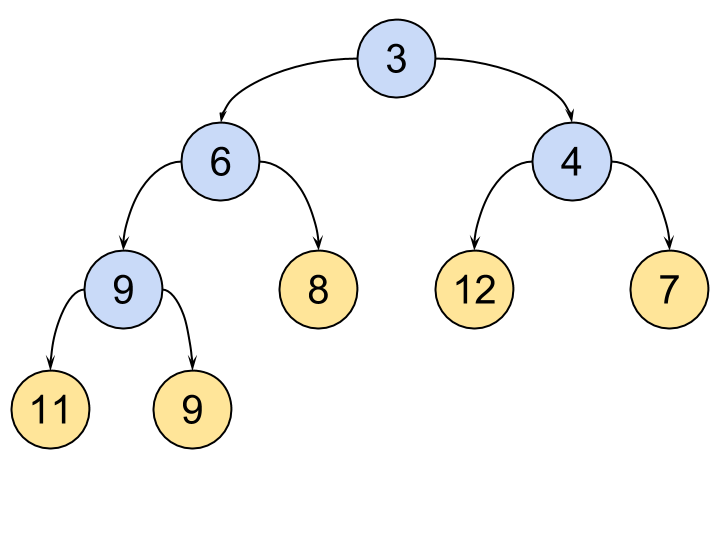
\includegraphics[height=5cm]{pics/30_1.png}
          \centering
      \end{figure}

      Удобнее всего двоичную кучу хранить в виде массива $>a[0..n-1]$, у которого нулевой элемент, $a[0]$ — элемент в корне, а потомками элемента $a[i]$ являются $a[2i+1]$ и $a[2i+2]$. Высота кучи определяется как высота двоичного дерева. То есть она равна количеству рёбер в самом длинном простом пути, соединяющем корень кучи с одним из её листьев. Высота кучи есть $O(\log{n})$, где $n$ — количество узлов дерева
    \end{definition}

    \begin{definition}{siftDown}
      Если значение измененного элемента увеличивается, то свойства кучи восстанавливаются функцией $ \mathrm {siftDown} $.

      Работа процедуры: если $i$-й элемент меньше, чем его сыновья, всё поддерево уже является кучей, и делать ничего не надо. В противном случае меняем местами $i$-й элемент с наименьшим из его сыновей, после чего выполняем $ \mathrm {siftDown} $ для этого сына.
      Процедура выполняется за время $O(\log{n})$.
    \end{definition}

    \begin{alg}
      Необходимо отсортировать массив $A$, размером $n$. Построим на базе этого массива за $O(n)$ кучу для максимума. Так как максимальный элемент находится в корне, то если поменять его местами с $A[n - 1]$, он встанет на своё место. Далее вызовем процедуру $ \mathrm{siftDown(0)} $, предварительно уменьшив $ \mathrm{heapSize} $ на $1$. Она за $O(\log{n})$ просеет $A[0]$ на нужное место и сформирует новую кучу (так как мы уменьшили её размер, то куча располагается с $A[0]$ по $A[n - 2]$, а элемент $A[n-1]$ находится на своём месте). Повторим эту процедуру для новой кучи, только корень будет менять местами не с $A[n - 1]$, а с $A[n-2]$.
      Делая аналогичные действия, пока $\mathrm{heapSize} $ не станет равен $1$, мы будем ставить наибольшее из оставшихся чисел в конец не отсортированной части. Очевидно, что таким образом, мы получим отсортированный массив.

      \begin{figure}[H]
          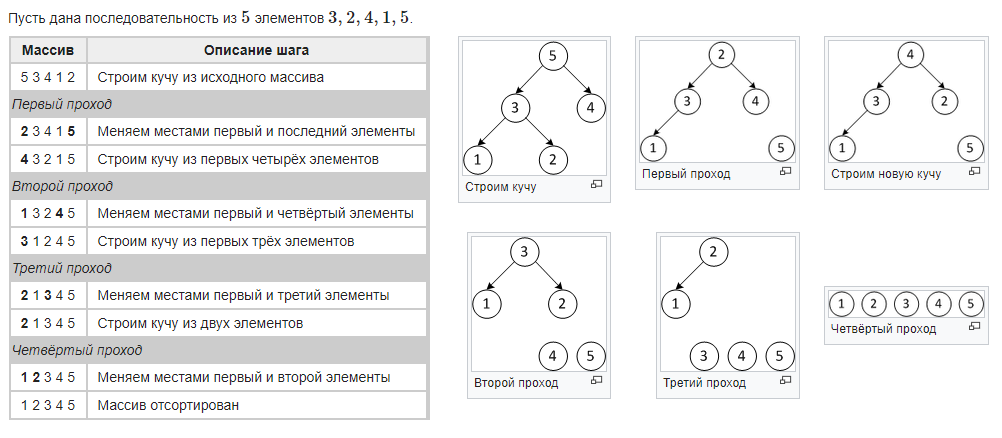
\includegraphics[width=15cm]{pics/30_2.png}
          \centering
      \end{figure}
    \end{alg}
  \end{enumerate}
\end{document}
